\chapter{La polarisation}
\section{État de polarisation}
On se rappelle que la notion d'onde est dérivée des équations de Maxwell
\begin{equation}
\rot\rot\vec{\mathcal{E}} = -\mu_0\epsilon_0\dfrac{\partial^2\vec{\mathcal{E}}}{\partial t^2}\qquad\Leftrightarrow
\qquad \Delta\mathcal{E}= \mu_0\epsilon_0\dfrac{\partial^2\mathcal{E}}{\partial t^2}
\end{equation}
où l'on a considéré une équation scalaire et non vectorielle par facilité : $\mathcal{E} = \mathcal{E}_x
,\mathcal{E}_y, \mathcal{E}_z$. Cette équation possède une solution d'onde plane 
\begin{equation}
\mathcal{E} = Ee^{ikz}e^{-i\omega t} + c.c.
\end{equation}
où on a considéré l'axe $z$ et où l'on n'a pas utilisé pour une fois les phaseurs mais une autre approche disant 
que le champ \textbf{réel}\footnote{Car on rajoute le complexe conjugué.} $\mathcal{E}$ n'est que le champ écrit 
sous forme de phaseur additionné à son complexe conjugué, c.c. Sous forme vectorielle
\begin{equation}
\vec{\mathcal{E}} = (E_x\vec{1_x}+E_y\vec{1_y}+E_z\vec{1_z})e^{ikz}e^{-i\omega t} + c.c.
\end{equation}
où les $E_i\in\mathbb{C}$ (ceci permet d'avoir un déphasage entre les composantes du champ). On sait que
\begin{equation}
\div \vec{\mathcal{E}} = ikE_z e^{ikz}e^{-i\omega t} = 0\qquad\Rightarrow\qquad E_z=0
\end{equation}

	\begin{wrapfigure}[11]{r}{3.5cm}
	\vspace{-5mm}
	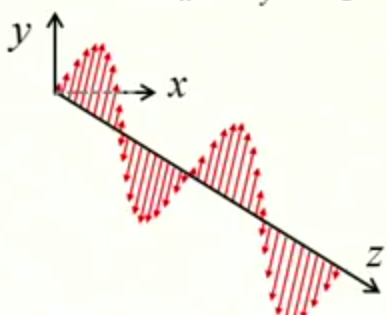
\includegraphics[scale=0.23]{ch5/image1.png}
	\captionof{figure}{ }
	\end{wrapfigure}
Une onde électromagnétique est dite \textit{transverse}
\begin{equation}
\hookrightarrow \vec{\mathcal{E}} = (E_x\vec{1_x}+E_y\vec{1_y})e^{ikz}e^{-i\omega t} + c.c.
\end{equation}
On observe bien sur le schéma ci-contre que l'amplitude possède une composante selon $x$ et $y$ : il 
s'agit d'une polarisation \textit{linéaire}.

	\subsection{Évolution du champ électrique d'une onde plane}
	Reprenons l'onde plane transverse se déplaçant le long de l'axe $z$
	\begin{equation}
	\vec{\mathcal{E}} = (E_x\vec{1_x}+E_y\vec{1_y})e^{ikz}e^{-i\omega t} + c.c.
	\end{equation}
	où $E_i\in\mathbb{C}$ : on peut les réécrire sous une forme polaire
	\begin{equation}
	E_x = \frac{1}{2}A_x e^{i\phi_x},\qquad\qquad E_y = \frac{1}{2}A_x e^{i\phi_y}
	\end{equation}
	où le facteur $1/2$ permet de faire apparaître un cosinus. 	Après substitution 
	(\danger\ ne pas oublier le c.c. sinon pas de cosinus et $\mathcal{E}\notin\mathbb{R}$ !)
	\begin{equation}
	\mathcal{E}_x = \frac{1}{2}A_x e^{i(kz-\omega t\phi_x)} + c.c.,\qquad\Leftrightarrow\qquad 
	\mathcal{E}_x = A_x\cos(kz-\omega t +\phi_x)
	\end{equation}
	On obtient similairement
	\begin{equation}
	\left\{\begin{array}{lll}
	\mathcal{E}_x &= A_x\cos(kz-\omega t +\phi_x) &= A_x\cos(\alpha)\\
	\mathcal{E}_y &= A_y\cos(kz-\omega t +\phi_y) &= A_y\cos(\alpha+\underbrace{\phi_y-\phi_x}_{\delta})\\
	\end{array}\right.
	\end{equation}
	
	\begin{wrapfigure}[9]{r}{4.5cm}
	\vspace{-9mm}
	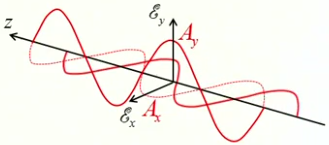
\includegraphics[scale=0.4]{ch5/image2.png}
	\captionof{figure}{ }
	\end{wrapfigure}
	Ceci représente une évolution du champ électrique, pas spécialement évidente à décrire. 
	En les traçant et en les sommant, on retrouve ci-contre pour $\phi_i=0$, l'évolution linéaire 
	(en pointillé ci-contre). 
	Si l'on considère $\phi_x\neq0$, $\phi_y=0$, il faut "reculer" le cosinus sur l'axe $z$ : on 
	a bien une avance de phase en $x$ (en trait plein ci-contre) et le champ ne s'annule plus nul 
	part.\\
	
	\begin{wrapfigure}[9]{l}{4cm}
	\vspace{-5mm}
	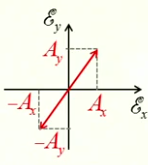
\includegraphics[scale=0.6]{ch5/image3.png}
	\captionof{figure}{ }
	\end{wrapfigure}	
	Pour se simplifier, posons que l'argument du cosinus dans l'expression de $\mathcal{E}_x$ est 
	$\alpha$ : il représente la distance parcourue sur l'axe $z$ si le temps est fixé, à une 
	constante près. Pour un $z$ donné, $\alpha$ représente le temps avec un signe moins et toujours 
	à une constante près. Prenons comme premier exemple, un déphasage nul $\delta = \phi_y-\phi_x=0$.
	Cherchons le lien entre $\mathcal{E}_x$ et $\mathcal{E}_y$ en effectuant le rapport suivant
	\begin{equation}
	\dfrac{\mathcal{E}_y}{\mathcal{E}_x} = \dfrac{A_y}{A_x}\qquad\Rightarrow\qquad \mathcal{E}_y = 
	\dfrac{A_y}{A_x}\mathcal{E}_x
	\end{equation}
	Cette linéarité est représentée ci-dessus. Les flèches représentent "l'oscillation" du champ 
	électrique. Il s'agit encore une fois de la \textit{polarisation linéaire} qui est caractérisée 
	par une certaine amplitude et un certain angle par rapport à l'axe.\\
	
	Considérons un autre exemple : $\delta=\phi_y-\phi_x=\frac{\pi}{2}$, soit un quart de période 
	de l'évolution des composantes. Cette situation ne donne aucun nœud, le champ ne s'annule plus.
	En substituant $\delta$
	\begin{equation}
	\left\{\begin{array}{ll}
	\mathcal{E}_x &= A_x\cos(\alpha)\\
	\mathcal{E}_y &= -A_y\sin(\alpha)
	\end{array}\right.
	\end{equation}
	En éliminant $\alpha$ de cette évolution paramétrique du champ, nous obtenons le lieu des points 
	qu'occupera le champ électrique :
	
 	\begin{wrapfigure}[5]{r}{3.2cm}
	\vspace{-5mm}
	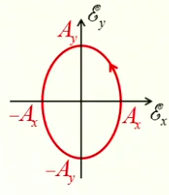
\includegraphics[scale=0.5]{ch5/image4.png}
	\captionof{figure}{ }
	\end{wrapfigure}	
	\begin{equation}
	\left(\frac{\mathcal{E}_x}{A_x}\right)^2+\left(\frac{\mathcal{E}_y}{A_y}\right)^2 = 1
	\end{equation}
	
	Il s'agit de l'équation d'une ellipse. Reste à savoir comment le champ agit dynamiquement : 
	dans quel sens "tourne-t-on" sur cette ellipse. Rappelons-nous : $\alpha = kz-\omega+\phi_x$. On 
	s'intéresse à la composante temporelle : si $z=\phi_x=0$, $\alpha \propto -t$. Quand le temps 
	évolue, on observe une diminution progressive de la composante en $x$ à partir de 1 et le comportement 
	inverse pour le composante en $y$, ayant un sinus. Le point de départ est 1 pour le cosinus et 0 
	pour le sinus, la rotation se fera dans le sens trigonométrique positif. Si l'on applique la 
	règle de la main droite pour déterminer la direction de l'axe $z$, les doigts vont dans le même 
	sens que la rotation sur l'ellipse : il s'agit d'une \textit{polarisation elliptique droite}.\\
	
 	\begin{wrapfigure}[7]{r}{5.5cm}
	\vspace{-5mm}
	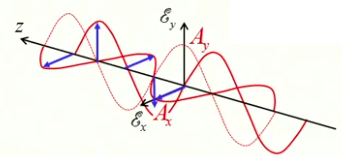
\includegraphics[scale=0.5]{ch5/image5.png}
	\captionof{figure}{ }
	\end{wrapfigure}	
	Regardons ceci géométriquement, en représentant les vecteurs résultants en bleu. On remarque 
	que si on effectue la règle de la main droite, en $z$, il tourne dans l'autre sens (le pouce 
	est opposé à l'axe $z$). C'est normal, l'évolution temporelle d'une onde progressive est inversée 
	par rapport à se composante spatiale. Un polarisation est dite \textit{droite} lorsqu'elle tourne 
	dans le sens horlogique lorsqu'on s'éloigne en $z$ : le sens de rotation en $z$ sera opposé à 
	sa rotation en $t$.\\
	
	Si $A_x=A_y$, on obtient une \textit{polarisation circulaire droite}. Si on considère $\delta = 
	-\frac{\pi}{2}$ on se trouve dans le cas d'un retard de phase. Le champ est spatialement 
	dextrogyre : il faut inverser le sens de la polarisation est alors dit \textit{gauche} (avec la
	règle de la main gauche, on obtiendrait l'axe $z$, petit moyen mnémotechnique).\\
	
	Cessons-en maintenant avec les exemples et considérons le cas général. Pour se faire, effectuons
	$\cos(a+b)$ dans l'expression $\mathcal{E}_y$
	\begin{equation}
	\frac{\mathcal{E}_x}{A_y} = \underbrace{\cos\alpha}_{\mathcal{E}_x/A_x}\cos\delta-\sin\alpha\sin\delta
	\end{equation}
	où l'on utilise la première expression (celle de $\mathcal{E}_x$) et le fait que $\DS \sin\alpha = 
	\sqrt{1-\left(\frac{\mathcal{E}_x}{A_x}\right)^2}$. On trouve alors
	\begin{equation}
	\frac{\mathcal{E}_y}{A_y} = \frac{\mathcal{E}_x}{A_x}\cos\delta -\sqrt{1-\left(\frac{\mathcal{E}_x}{
	A_x}\right)^2}\sin\delta
	\end{equation}
	N'ayant plus de $\alpha$, il s'agit bien du lieu des points de l'extrémité du vecteur du champ électrique. 
	Analysons ceci en commençant par passer la racine à gauche et en élevant tout au carré
	\begin{equation}
	\sqrt{1-\left(\frac{\mathcal{E}_x}{A_x}\right)^2}\sin\delta = \frac{\mathcal{E}_x}{A_x}\cos\delta -
	\frac{\mathcal{E}_y}{A_y} 
	\end{equation}
	Dès lors, en effectuant le produit remarquable
	\begin{equation}
	\left[1-\left(\frac{\mathcal{E}_x}{A_x}\right)\right]\sin^2\delta = \left(\frac{\mathcal{E}_x}{A_x}\right)^2
	\cos^2\delta +\left(\frac{\mathcal{E}_y}{A_y}\right)^2- 2\frac{\mathcal{E}_x\mathcal{E}_y}{A_xA_y}\cos\delta
	\end{equation}
	En simplifiant l'identité fondamentale trigonométrique
	\begin{equation}
	\sin^2\delta = \left(\frac{\mathcal{E}_x}{A_x}\right)^2
	+\left(\frac{\mathcal{E}_y}{A_y}\right)^2- 2\frac{\mathcal{E}_x\mathcal{E}_y}{A_xA_y}\cos\delta
	\end{equation}
	
		\begin{wrapfigure}[2]{r}{4.5cm}
	\vspace{-12mm}
	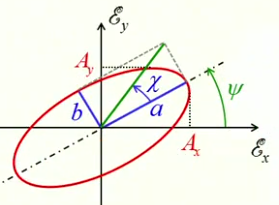
\includegraphics[scale=0.5]{ch5/image6.png}
	\captionof{figure}{ }
	\end{wrapfigure}
	Il s'agit de l'équation d'une conique qui n'est rien d'autre qu'une ellipse. Il s'agit du cas de 
	polarisation le plus général portant le doux nom d'\textit{ellipse de polarisation}. Celle-ci aura 
	une certaine inclinaison $\psi$ repérée par rapport à l'axe $x$. Sans rentrer dans les détails, on 
	peut montrer que
	\begin{equation}
	\psi = \frac{1}{2}\arctan\left[\dfrac{2A_xA_y}{A_x^2-A_y^2}\cos\delta\right]
	\end{equation}
	La différence avec les secondaires et qu'à la place d'utiliser $a$ et $b$ pour le grand/petit axe, 
	on utilise l'ellipticité $\chi$ donné par (non démontré ici)
	\begin{equation}
	\chi = \frac{1}{2}\arcsin\left[\dfrac{2A_xA_y}{A_x^2+A_y^2}\sin\delta\right]
	\end{equation}
	L’ellipse de polarisation, et donc l'état de polarisation, sera décrite par son inclinaison et 
	son ellipticité. Par construction $\chi=\arctan(b/a)$ où $|b|<a$ (si $b>0$ la polarisation sera 
	droite) et donc $|\chi| \leq  \frac{\pi}{4} \rightarrow \chi <0$ représente une polarisation 
	elliptique gauche.\\
	
	Prenons un exemple : $\delta = 0\rightarrow \chi = 0\rightarrow b = 0$ et l'ellipse se réduit à 
	une droite. Une ellipticité nulle indique que l'on se trouve dans le cadre d'une polarisation 
	linéaire. Pour l'inclinaison 
	\begin{equation}
	\tan(2\psi) = \left[\frac{2A_y/A_x}{1-A_y^2/A_x^2}\right] = \dfrac{2\tan\psi}{1-\tan^2\psi}
	\end{equation}
	où l'on a utilisé la formule de l'angle double. Par identification $A_y/A_x = \tan\psi$ ce qui 
	est bien le résultat précédemment obtenu.\\
	
	\begin{wrapfigure}[6]{l}{4cm}
	\vspace{-9mm}
	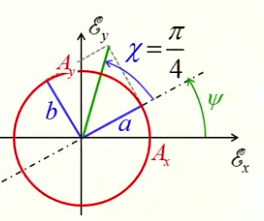
\includegraphics[scale=0.34]{ch5/image7.png}
	\captionof{figure}{ }
	\end{wrapfigure}
	Soif de savoir, partons sur un nouvel exemple : $\delta = \frac{\pi}{2}, A_y=A_x \rightarrow 
	\chi = \frac{\pi}{4}\rightarrow a=b=A_x$. Il s'agit de la polarisation circulaire droite, 
	$\chi$ étant positif. Pour le calcul de l'inclinaison, on obtient une indétermination ($\psi = 0/0$)
	ce qui est cohérent : l'inclinaison d'un cercle est indéterminée. La fin de la vidéo propose quelques 
	petites illustrations animées.\\
	
	Même si ces expressions sont correctes, elles sont peut utilisables en pratique. La section 
	suivante se consacre dès lors à la mesure expérimentale de la polarisation.
	
	\newpage
\section{Mesure de la polarisation}
Les mesures sur la lumières sont essentiellement des mesures de l'intensité
\begin{equation}
I = A_x^2+A_y^2
\end{equation}
Avant de voir comment mesurer ceci, intéressons-nous au lien entre $\psi$ et $\chi$. Nous avions
\begin{equation}
\left\{\begin{array}{ll}
\psi &= \frac{1}{2}\arctan\left[\dfrac{2A_xA_y}{A_x^2-A_y^2}\cos\delta\right]\\
\chi &= \frac{1}{2}\arcsin\left[\dfrac{2A_xA_y}{A_x^2+A_y^2}\sin\delta\right]	
\end{array}\right.
\end{equation}
En manipulant ces expressions (en faisant surtout l'effort de le faire), il est possible de 
ré-exprimer $A_x$ (en remplaçant l'expression de $I$ dans $\chi$), de même pour $A_y$.
En élevant ces deux expressions au carré on retrouve bien les deux relations suivantes 
\begin{equation}
\left\{\begin{array}{ll}
I &= A_x^2+A_y^2\\
A_x^2-A_y^2 &= I\cos(2\chi)\cos(2\psi)
\end{array}\right.
\end{equation}
Les angles doubles apparaissant dans cette dernière expression justifie l'utilité de 
l'utilisation de $\chi$.

	\subsection{Sphère de Poincaré}
	Ces relations remarquables faisant intervenir les angles $\psi$ et $\chi$ a donné l'idée à 
	Poincaré de représenté les états de polarisation sous la forme d'un point sur une sphère. 
	
	\begin{center}
	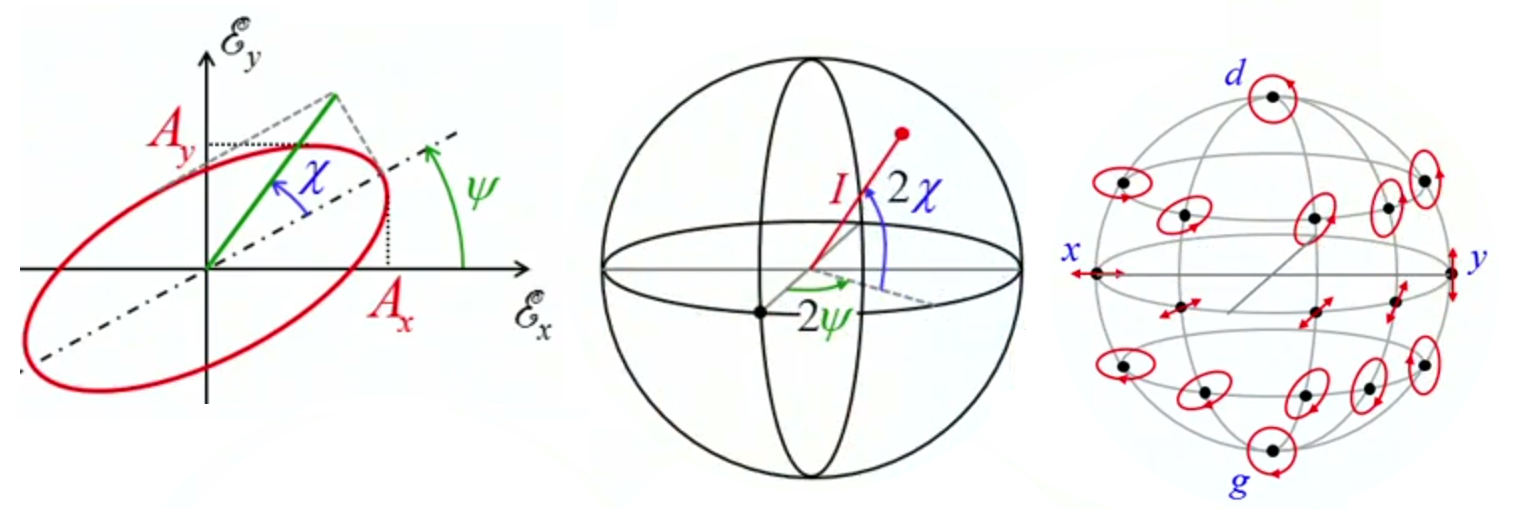
\includegraphics[scale=0.30]{ch5/image8.png}
	\captionof{figure}{ }
	\end{center}
	
	Un point sur cette sphère est repéré à partir de deux angles : $2\psi$ comme angle polaire et 
	$2\chi$ comme angle azimutal. On pourrait croire que le facteur 2 est limitant, mais ce n'est 
	pas le cas car pour un angle $\chi>180^\circ$ on retrouve les mêmes états.\\
	
	\begin{wrapfigure}[5]{l}{3.64cm}
	\vspace{-9mm}
	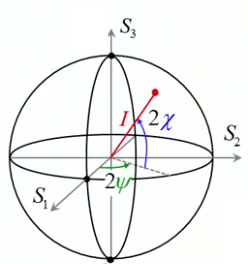
\includegraphics[scale=0.34]{ch5/image9.png}
	\captionof{figure}{ }
	\end{wrapfigure}
	L'intérêt de cette représentation vient de George Stokes : il a proposé de représenté l'état 
	de polarisation, soit un point de la sphère de Poincaré, en terme de coordonnées dans un système 
	cartésien à l'aide des paramètres de Stokes $S_1, S_2$ et $S_3$. La sphère de Poincaré est donc 
	maintenant décrite dans ce repère cartésien. Notons que cette sphère a pour rayon l'intensité de 
	la lumière émise et bien qu'il n'est pas nécessaire à la caractérisation de la polarisation, 
	c'est toujours utile de l'avoir. On désigne l'intensité avec le paramètre de Stokes $S_0$.
 	\begin{equation}
 	S_0 = I
 	\end{equation}
 	Le premier paramètre de Stokes est la coordonnée $S_1$ qui est obtenue en projetant le "vecteur 
 	intensité" dans le plan horizontal $S_1S_2$ puis en effectuant la projection sur $S_1$ (\danger\ 
 	l'angle $\chi$ n'est pas exactement défini comme les coordonnées polaires). En faisant de même 
 	pour $S_2$ et $S_3$, on obtient les \textit{paramètres de Stokes}
 	\begin{equation}
	\left\{\begin{array}{ll}
	S_0 &= I\\
 	S_1 &= I\cos(2\chi)\cos(2\psi)\\
 	S_2 &= I\cos(2\chi)\sin(2\psi)\\
 	S_3 &= I\sin(2\chi)
	\end{array}\right.
 	\end{equation}
 	Il est évident que la somme des composantes au carrée va donner la norme au carrée du vecteur 
 	intensité, étant dans un repère cartésien
 	\begin{equation}
 	S^2_1+S^2_2+S^2_3 = S^2_0
 	\end{equation}
	On peut maintenant revenir à nos deux expressions précédentes
	\begin{equation}
	\left\{\begin{array}{ll}
	A_x &= \sqrt{\frac{I}{2}}[1+\cos(2\chi)\cos(2\psi)]^{\frac{1}{2}}\\
	A_y &= \sqrt{\frac{I}{2}}[1-\cos(2\chi)\cos(2\psi)]^{\frac{1}{2}}
	\end{array}\right.
	\end{equation}
	Et on va voir que des regroupements vont être possibles avec les paramètres de Stokes. 
 	\begin{equation}
	\left\{\begin{array}{lll}
	S_0 &= I&\qquad\rightarrow S_0 = A_x^2+A_y^2\\
 	S_1 &= I\cos(2\chi)\cos(2\psi)&\qquad\rightarrow S_1 = A_x^2-A_y^2\\
 	S_2 &= I\cos(2\chi)\sin(2\psi)&\qquad\rightarrow S_2 = 2A_xA_y\cos\delta\\
 	S_3 &= I\sin(2\chi)&\qquad\rightarrow S_3 = 2A_xA_y\sin\delta
	\end{array}\right.
 	\end{equation}
 	Les démonstrations ne sont pas données ici, mais il suffit de partir des expressions de 
 	ci-dessus et faire un peu d'algèbre.
 	
 		\subsubsection{Illustration}
 		Considérons quelques exemples pour s'habituer à ce nouveau formalisme. Regardons la 
 		situation aux deux pôles : $S_1=S_2=0$. On peut directement en tirer que
 		\begin{equation}
 		A_x = A_y,\qquad\qquad \delta = \pm\frac{\pi}{2}
 		\end{equation}
		Comme $A_x=A_y$, $S_3 = 2\underbrace{A_xA_y}_{\pm I}\sin\delta = \pm I$ en utilisant 
		l'expression $S_0 = A_x^2+A_y^2 = 2A_x = I$. En en tire $\chi = \pm \frac{\pi}{4}$. 
		Comme nous avons une indétermination sur $\psi$ (dans l'expression de $S_2$, peu 
		importe sa valeur tout est vérifié) il s'agit bien d'un état de polarisation circulaire. \\
		
		Autre exemple : à l'équateur $S_3=0 \rightarrow \chi = 0 \rightarrow \delta = 0\rightarrow 	
		2A_xA_y=I\sin(2\psi)$. Avec $S_1$ : $A_x^2-A_y^2 = I\cos(2\psi)$. En faisant le rapport des 
		deux, on retrouve $\tan(2\psi)=\frac{2A_xA_y}{A_x^2-A_y^2}$, c'est bien la polarisation 
		linéaire précédemment rencontrée.
		
	\subsection{Mesure de l'état de polarisation}
	Imaginons qu'une lumière ai une certaine polarisation et qu'il est nécessaire de la déterminer 
	la polarisation. Nous allons pouvoir tout déterminer, à l'aide de quatre étapes 
	\begin{enumerate}
	\item \textit{Étape "0"}\\
	Il suffit de mesurer l'intensité de la lumière
	\begin{equation}
	I_0 = A_x^2+A_y^2 = S_0
	\end{equation}
	\item \textit{Étape "1"}\\
	Il faut préalablement insérer un polarisateur mis en polarisation horizontale. Se faisant, 
	nous récupérons l'intensité en $x$, $I_1=A_x^2$. 
	\begin{center}
	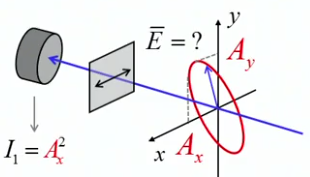
\includegraphics[scale=0.50]{ch5/image11.png}
	\captionof{figure}{ }
	\end{center}	
	Avec cette mesure, il est possible d'effectuer 
	une manipulation intéressante
	\begin{equation}
	I_0-I_1 = A_y^2
	\end{equation}
	En peut en déduire $S_1$
	\begin{equation}
	\hookrightarrow S_1 = I_1(I_0-I_1) = 2I_1-I_0
	\end{equation}
	\item \textit{Etape "2"}\\
	Cette étape consiste à incliner le polariseur à 45$^\circ$. Il est important de bien comprendre 
	ce qui se passe dans le polariseur : la vibration $\mathcal{E}_x$ incidente peut être vue comme 
	la combinaison d'une vibration dans l'axe perpendiculaire à l'axe du polariseur  et une vibration 
	parallèle à cette axe (principe de superposition). 
	\begin{center}
	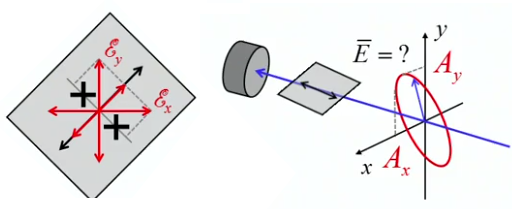
\includegraphics[scale=0.50]{ch5/image12.png}
	\captionof{figure}{ }
	\end{center}		
	La vibration perpendiculaire à l'axe du polariseur 
	se fait absorbé par celui-ci, seule la composante parallèle à l'axe passera dont l'intensité sera 
	$\frac{1}{2}=\left(\frac{1}{\sqrt{2}}\right)^2$ (car 45$^\circ$)  de celle incidente. Un raisonnement similaire peut être tenu 
	pour $\mathcal{E}_y$. On mesurera alors
	\begin{equation}
	I_2 = \left|\dfrac{1}{\sqrt{2}}A_xe^{i\phi_x}+\dfrac{1}{\sqrt{2}}A_ye^{i(\phi_x+\delta)}\right|^2 = 
	\frac{1}{2}|A_x + A_y(\cos\delta +i\sin\delta)|^2
	\end{equation}
	où on a supprimé tous les termes "semblables". En effectuant le module carré
	\begin{equation}
	A_x^2+2A_xA_y\cos\delta + A_y^2\cos^2\delta + A_y^2\sin^2\delta  
	\end{equation}
	On trouve alors
	\begin{equation}
	I_2 = \frac{1}{2}\left[A_x^2+A_y^2+2A_xA_y\cos\delta\right]\quad \Rightarrow\quad 2I_2 = 
	I_0+S_2
	\end{equation}
	où les $1/2$ vient des $1/\sqrt{2}$. Finalement
	\begin{equation}
	S_2 = SI_2 - I_0
	\end{equation}
	\item \textit{Étape "3"}\\
	Pour obtenir le dernier paramètre, il est nécessaire d'introduire une lame quart d'onde. Il 
	s'agit d'une lame biréfringente : il possède deux indices de réfraction en fonction de la 
	direction. Une composante accumulera une certaine phase causant ici un déphasage entre nos 
	deux composantes du champ électrique. 
	\begin{center}
	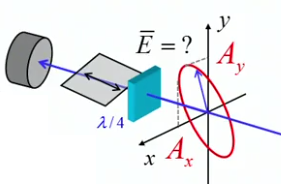
\includegraphics[scale=0.50]{ch5/image13.png}
	\captionof{figure}{ }
	\end{center}	
	Au départ d'un déphasage nul (polarisation linéaire) 
	on obtient  un déphasage $\phi_y-\phi_x=-\frac{\pi}{2}$ (soit $\lambda/4$, d'où le nom).  
	Ceci correspond à une polarisation circulaire gauche. En terme de mesure, il faut tenir 
	compte de ce déphasage supplémentaire
	\begin{equation}
	I_3 = \left|\dfrac{1}{\sqrt{2}}A_xe^{i\phi_x}+\dfrac{1}{\sqrt{2}}A_ye^{i\left(\phi_x+\delta-
	\frac{\pi}{2}\right)}\right|^2 = \frac{1}{2}|A_x + A_y(-i\cos\delta +\sin\delta)|^2
	\end{equation}
	En calculant le module carré
	\begin{equation}
	|A_x + A_y(-i\cos\delta +\sin\delta)|^2 = A_x^2+2A_xA_y\sin\delta + A_y^2\sin^2\delta +A_y^2
	\cos^2\delta
	\end{equation}
	Avec l'identité trigonométrique fondamentale, on trouve
	\begin{equation}
	I_3 = \frac{1}{2}[A_x^2+A_y^2+2A_xA_y\sin\delta]
	\end{equation}
	où l'on voit apparaître le paramètre $S_3$. On obtient alors
	\begin{equation}
	S_3 = 2I_3-I_0
	\end{equation}
	\end{enumerate}
	Nous voyons que ces quatre étapes permettent d'accéder facilement de façon expérimentales à ces 
	paramètres de Stokes. Ceci n'est que une des multiples techniques possible pour mesurer une 
	polarisation : une autre technique - directement inspirée de celle-ci - sera vue en séance de 
	laboratoire. Le gros désavantage de cette méthode est que le placement d'un polariseur provoque 
	tout de même une atténuation en $x$. Il faudrait quelque peu corriger ces mesures : il existe 
	d'autres moyen de caractériser la polarisation, ce que nous aurons l'occasion de voir plus tard.
	
	
\newpage
\section{Formalisme de Jones}
Ce formalisme se base sur la représentation complexe du champ électrique
\begin{equation}
\vec{\mathcal{E}} = (E_x\vec{1_x}+E_y\vec{1_y})e^{ikz}e^{-i\omega t} + c.c.\qquad\text{où }\ E_x = 
\frac{1}{2}A_xe^{i\phi_x},\quad E_y = \frac{1}{2}A_ye^{i\phi_y}
\end{equation}
Le premier terme n'est en réalité pas vraiment un phaseur. De plus, on remarque que l'amplitude 
$E_i$ n'est que la moitié de l'amplitude réelle. Ce choix de notation a été fait pour se rapprocher 
de la littérature scientifique, mais rien n'empêche d'utiliser les fameux phaseurs
\begin{equation}
\underline{\vec{\mathcal{E}}} = (\underline{E_x}\vec{1_x}+\underline{E_y}\vec{1_y})e^{ikz}e^{-i\omega t}\qquad\text{où }\ \underline{E_x} = A_xe^{i\phi_x},\quad \underline{E_y} = A_ye^{i\phi_y}
\end{equation}
Si ici nous passons en phaseurs, c'est parce que le formalisme de Jones a été développé avec un 
tel outil. Lorsque l'on parle de $\underline{\vec{\mathcal{E}}}$, cela désigne bien un phaseur. Le 
champ sera alors obtenu en considérant la partie réelle de ce phaseur\footnote{C'est semblable avec 
ce que l'on faisait en ajoutant +c.c. où l'on prenait deux fois la partie réelle, d'où le facteur 
1/2 dans l'amplitude.}.\\

L'état de polarisation générale est elliptique d'inclinaison $\psi$ et d'ellipticité $\chi$. Le 
formalisme de Jones est utile d'un point de vue théorique, contrairement à la précédente section. 
Il permet de décrire d'un point de vue théorique l'évolution de la polarisation dans les systèmes 
optiques. Jones propose d'écrire le vecteur amplitude sous la forme vectorielle 
\begin{equation}
\left(\begin{array}{c}
\underline{E_x}\\
\underline{E_y}
\end{array}\right) = \left(\begin{array}{c}
A_xe^{i\phi_x}\\
A_ye^{i\phi_y}
\end{array}\right)
\end{equation}

		\begin{wrapfigure}[4]{l}{5.5cm}
	\vspace{-4mm}
	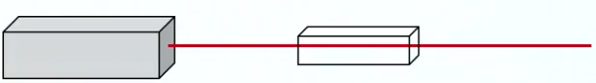
\includegraphics[scale=0.25]{ch5/image14.png}
	\captionof{figure}{ }
	\end{wrapfigure}
Il s'agit du \textit{vecteur de Jones}. Ce n'est rien d'autre qu'une notation plus compacte de 
notre vecteur en vue de bénéficier d'un formalisme matriciel : l'action d'un dispositif optique 
va pouvoir être exprimé sous forme d'une matrice
\begin{equation}
\left(\begin{array}{c}
\underline{E_x'}\\
\underline{E_y'}
\end{array}\right) = \left(\begin{array}{cc}
a & b\\
c & d
\end{array}\right)\left(\begin{array}{c}
\underline{E_x}\\
\underline{E_y}
\end{array}\right)
\end{equation}

\subsection{Matrice de Jones}
	\subsubsection{Propagation libre}
Afin d'introduire ce formalisme, commençons par un cas quelque peu trivial : la propagation libre. 
Le système optique est l'espace entre $0$ et $L$. 
\begin{center}
	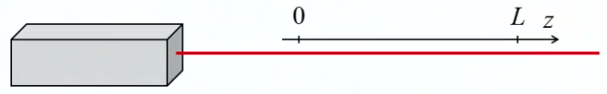
\includegraphics[scale=0.35]{ch5/image15.png}
	\captionof{figure}{ }
\end{center}
La matrice de Jones sera simple : il faut utiliser 
un propagateur pour une distance $L$ sur chaque composante de notre vecteur de Jones
\begin{equation}
\left(\begin{array}{c}
\underline{E_x'}\\
\underline{E_y'}
\end{array}\right) = \left(\begin{array}{cc}
e^{ikL} & 0\\
0 & e^{ikL}
\end{array}\right)\left(\begin{array}{c}
\underline{E_x}\\
\underline{E_y}
\end{array}\right) = e^{ikL}\left(\begin{array}{cc}
1 & 0\\
0 & 1
\end{array}\right)\left(\begin{array}{c}
\underline{E_x}\\
\underline{E_y}
\end{array}\right)
\end{equation}
La matrice identité $\mathcal{I}$ montre que l'on n'a pas modifié l'état de polarisation. On retrouve 
l'état de polarisation à la sortie.

\subsubsection{Polariseur}
Considérons maintenant un polariseur horizontal. La matrice d'un tel polariseur sera la suivante
\begin{equation}
\left(\begin{array}{c}
\underline{E_x'}\\
\underline{E_y'}
\end{array}\right) = \left(\begin{array}{cc}
1 & 0\\
0 & 0
\end{array}\right)\left(\begin{array}{c}
\underline{E_x}\\
\underline{E_y}
\end{array}\right) = \left(\begin{array}{c}
\underline{E_x}\\
0
\end{array}\right)
\end{equation}
Ce résultat est évident dans le sens ou nous savons que seul la composante selon $x$ sera transmise.
	
		\subsubsection{Lame de phase}
		Une lame de phase pourrait être une lame demi ou quart d'onde. Ici, on se doute que la matrice 
		sera (vraiment juste) un peu plus compliquée.
		\begin{equation}
		\left(\begin{array}{c}
		\underline{E_x'}\\
		\underline{E_y'}
		\end{array}\right) = \left(\begin{array}{cc}
		1 & 0\\
		0 & e^{i\delta}
		\end{array}\right)\left(\begin{array}{c}
		\underline{E_x}\\
		\underline{E_y}
		\end{array}\right)= \left(\begin{array}{c}
		\underline{E_x}\\
		\underline{E_y}e^{i\delta}
		\end{array}\right)
		\end{equation}
		Rappelons que ce qui est intéressant c'est bien le déphasage entre les deux composantes 
		et non la phase à un point $z$ précis.
		
		\textbf{Remarque :} Pour lame $\lambda/4$, $\delta = \pi/2$ alors que pour une lame $\lambda/2$, $\delta = \pi$
		
		\subsubsection{Rotation}
		La rotation de la polarisation est quelque chose d'important. Pour se faire, introduisons 
		les axes $x$ et $y$. Considérons une polarisation en $x$ et on considère un système causant 
		une rotation $\alpha$ à notre faisceau en $x$ (par exemple, un verre d'eau sucrée (du à la 
		chiralité de la molécule de sucre).
	\begin{center}
	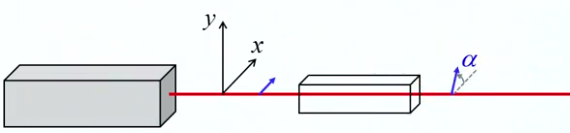
\includegraphics[scale=0.35]{ch5/image17.png}
	\captionof{figure}{ }
\end{center}			
	 Trouvons cette matrice en étudiant des cas particuliers. 
		Nous avons une polarisation en $x$ comme entrée et comme sortie une rotation de $\alpha$
		\begin{equation}
		\left(\begin{array}{c}
		1\\
		0
		\end{array}\right),\qquad\qquad		\left(\begin{array}{c}
		\cos\alpha\\
		\sin\alpha
		\end{array}\right)
		\end{equation}
		Forcément, notre matrice doit vérifier
		\begin{equation}
			\left(\begin{array}{c}
		1\\
		0
		\end{array}\right) = \left(\begin{array}{cc}
		\cos\alpha & b\\
		\sin\alpha & d
		\end{array}\right)\left(\begin{array}{c}
		\underline{E_x}\\
		\underline{E_y}
		\end{array}\right)= \left(\begin{array}{c}
		\cos\alpha\\
		\sin\alpha
		\end{array}\right)
		\end{equation}
		où $b,d$ sont à déterminer. En considérant cette fois une polarisation verticale et la sortie
		\begin{equation}
				\left(\begin{array}{c}
		1\\
		0
		\end{array}\right),\qquad\qquad		\left(\begin{array}{c}
		-\sin\alpha\\
		\cos\alpha
		\end{array}\right)
	\end{equation}				
	Nous avons ainsi trouvé notre matrice de rotation. Dans le formalisme de Jones :
	\begin{equation}
			\left(\begin{array}{c}
		\underline{E_x'}\\
		\underline{E_y'}
		\end{array}\right) = \left(\begin{array}{cc}
	\cos\alpha & -\sin\alpha\\
	\sin\alpha & \cos\alpha
	\end{array}\right)\left(\begin{array}{c}
		\underline{E_x}\\
		\underline{E_y}
		\end{array}\right)
	\end{equation}
	
		\subsubsection{Rotation d'un élément}
		Illustrons le cas de la rotation d'une lame d'onde\footnote{Le polariseur est laissé comme 
		exercice.} Comme nous ne savons pas comment décrire une lame d'onde inclinée de $\alpha$ nous 
		allons ruser : on va redresser la lame mais tourner la polarisation dans l'autre sens. En effet, 
		entre l'axe de la lame et la polarisation se trouve un angle $-\alpha$. 
\begin{center}
	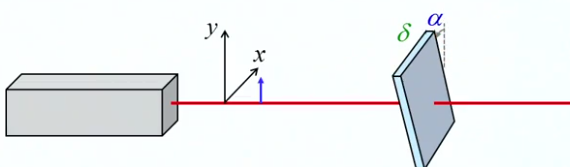
\includegraphics[scale=0.35]{ch5/image16.png}
	\captionof{figure}{ }
\end{center}		
		En redressant tout, 
		la lame va redevenir horizontale et la polarisation va tourner d'un angle $-\alpha$. Faisant 
		ceci, on pourra appliquer la matrice pour la lame de phase et obtenir une sortie. Il faut alors 
		redresser cette sortie d'un angle $\alpha$.
		\begin{center}
	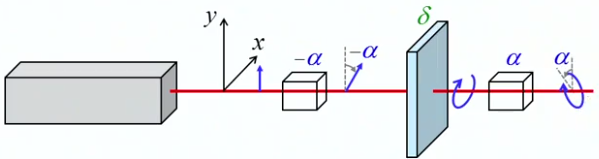
\includegraphics[scale=0.35]{ch5/image18.png}
	\captionof{figure}{ }
\end{center}	
		Matriciellement, cela donne
		\begin{equation}
		\left(\begin{array}{c}
		\underline{E'}_x\\
		\underline{E'}_y
		\end{array}\right)\left(\begin{array}{cc}
	\cos\alpha & -\sin\alpha\\
	\sin\alpha & \cos\alpha
	\end{array}\right)
	\left(\begin{array}{cc}
	1 & 0\\
	0 & e^{i\delta}
	\end{array}\right)\left(\begin{array}{cc}
	\cos\alpha & \sin\alpha\\
	-\sin\alpha & \cos\alpha
	\end{array}\right)		\left(\begin{array}{c}
		\underline{E}_x\\
		\underline{E}_y
		\end{array}\right)
		\end{equation}
		Une lame inclinée d'une angle $\alpha$ est représentée par les trois matrices ci-dessus : 
		la matrice de rotation opposé $-\alpha$, la matrice de la lame suivi de la matrice de rotation de 
		l'angle de la lame, $\alpha$.\\
		
		\textsc{Illustration 1}\ \\
		Supposons que nous plaçons à la sortie d'un laser un polariseur horizontal suivi d'une 
		lame demi-onde inclinée d'un angle $\alpha$. 
		\begin{center}
	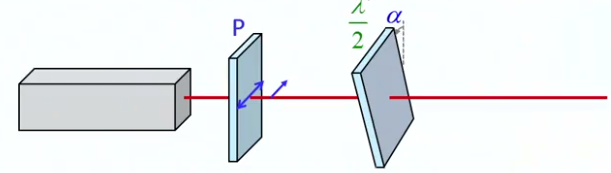
\includegraphics[scale=0.35]{ch5/image19.png}
	\captionof{figure}{ }
\end{center}			
		La polarisation induite par le polariseur 
		revient à considérer que, à l'entrée de la lame
		\begin{equation}
		\left(\begin{array}{c}
		\underline{E}_x\\
		\underline{E}_y
		\end{array}\right) = \left(\begin{array}{c}
		1\\
		0
		\end{array}\right)
		\end{equation}
		Pour une lame demi-onde, $\delta =\pi \rightarrow e^{i\pi} = -1$. Nous obtenons alors
		\begin{equation}
				\left(\begin{array}{c}
		\underline{E'}_x\\
		\underline{E'}_y
		\end{array}\right)\left(\begin{array}{cc}
	\cos\alpha & -\sin\alpha\\
	\sin\alpha & \cos\alpha
	\end{array}\right)
	\left(\begin{array}{cc}
	1 & 0\\
	0 & -1
	\end{array}\right)\left(\begin{array}{cc}
	\cos\alpha & \sin\alpha\\
	-\sin\alpha & \cos\alpha
	\end{array}\right)		\left(\begin{array}{c}
		1\\
		0
		\end{array}\right)
		\end{equation}
		Après avoir effectué les produits matriciels, nous trouvons
		\begin{equation}
		\left(\begin{array}{c}
		\underline{E'}_x\\
		\underline{E'}_y
		\end{array}\right) = \left(\begin{array}{cc}
		cos^2\alpha - \sin^2\alpha\\
		2\sin\alpha\cos\alpha
		\end{array}\right)
		\end{equation}
		En appliquant les formules trigonométrique de l'arc double, on obtient
		\begin{equation}
		\left(\begin{array}{c}
		\underline{E'}_x\\
		\underline{E'}_y
		\end{array}\right)		\left(\begin{array}{cc}
		\cos(2\alpha)\\
		\sin(2\alpha)
		\end{array}\right)
		\end{equation}
		L'effet d'une lame demi-onde sur une polarisation linéaire revient à tourner 
		celle-ci d'un angle $2\alpha$.\\
		
		
		\textsc{Illustration 2}\ \\
		Considérons cette-fois une polarisation linéaire inclinée à $45^\circ$ incidente sur 
		une lame quart d'onde verticale. Nous avons premièrement
		\begin{equation}
		\left(\begin{array}{c}
		\underline{E}_x\\
		\underline{E}_y
		\end{array}\right) = \left(\begin{array}{c}
		1/\sqrt{2}\\
		1/\sqrt{2}
		\end{array}\right)
		\end{equation}
		où ce vecteur de Jones a été normalisé. Pour une lame quart d'onde $\delta = \frac{\pi}{2} 
		\Rightarrow e^{i\delta} =i$ de sorte à obtenir
		\begin{equation}
		\left(\begin{array}{c}
		\underline{E'}_x\\
		\underline{E'}_y
		\end{array}\right)		\left(\begin{array}{cc}
		1 & 0\\
		0 & i
		\end{array}\right)\left(\begin{array}{c}
		1/\sqrt{2}\\
		1/\sqrt{2}
		\end{array}\right) = \dfrac{1}{\sqrt{2}}\left(\begin{array}{c}
		1\\
		i
		\end{array}\right)
		\end{equation}
		Rappelons-nous que les composantes du vecteur sont les amplitudes en $x$ et $y$ de notre onde :
		\begin{equation}
		\underline{\vec{\mathcal{E}}} = (\underline{E_x}\vec{1_x}+\underline{E_y}\vec{1_y})e^{ikz}e^{-i
		\omega t}
		\end{equation}
		Dans notre cas $\underline{E_x}=1$ et $\underline{E_y} = i$, ce qui donne bien un déphasage de 
		$\frac{\pi}{2}$ entre les deux champs. Ceux-ci sont donc en quadrature de phase, la polarisation 
		est circulaire droite, la phase en $y$ ayant été avancée. Le vecteur de Jones normalisé d'une 
		polarisation circulaire droite est donné par
		\begin{equation}
		\dfrac{1}{\sqrt{2}}\left(\begin{array}{c}
		1\\
		i
		\end{array}\right)
		\end{equation}
		Pour une polarisation circulaire gauche, il suffit de remplacer $i$ par $-i$, $\delta$ valant 
		$-\pi/2$.\\
		\\
		
		
		

			\begin{center}
	
\includegraphics[scale=0.15]{ch5/fin}
	%\captionof{figure}{ }
\end{center}				
	
	
	
	
	
	
	
	
	
	
	
	
	
	
	
	
